\documentclass[12pt,a4,english,finnish,pdflatex%,handout
]{beamer}
\definecolor{MyGreen}{RGB}{50, 120, 50}
\usecolortheme[named=MyGreen]{structure}

\usepackage{babel}
\usepackage[utf8]{inputenc}
\usepackage[T1]{fontenc}
\usepackage{amsmath,amssymb} 
\usepackage{animate}
\usepackage{multimedia}

\usepackage{natbib}
\bibpunct[: ]{(}{)}{,}{}{}{;}

\usepackage{tikz}

\usepackage{tipa}

\usepackage{hyperref}

\setbeamertemplate{navigation symbols}{}

\graphicspath{{figures/}}

\setlength{\leftmargini}{0pt}
\setlength{\leftmarginii}{1em}

\newcommand{\kommentti}[1]{
  {\bf[#1]}
}



\begin{document}
\title{Kieliultraääniprojekteja ja analyysimenetelmiä\\
  a.k.a. UltraLuento 2.
} 
\author{Pertti Palo} 
\date{14. huhtikuuta 2023}

\frame{\titlepage
} 

\frame{\frametitle{Edellisen kerran sisältöä}
  \begin{itemize}
  \item 1. Luento: Ultraäänikuvauksen ominaisuudet ja toimintaperiaate
    \begin{itemize}
    \item Etuja
    \item Epäideaalisuuksia (eli puutteita)
    \item Fyysinen toimintaperiaate
    \end{itemize}
  \item 1. Luento: Puheartikulaation mittaaminen ultraäänellä
    \begin{itemize}
    \item Miltä kuva näyttää?
    \end{itemize}
  \end{itemize}

  \vfill
  \bf \Large 
  \usebeamercolor[fg]{title}
  Onko uusia tai vanhoja kysymyksiä?
}

\frame{\frametitle{2. UltraLuento: Ultraäänellä tallennetun puhemateriaali ja analyysi}

\begin{itemize}
    \item Osa I: Projekti- ja analyysiesimerkkejä
    \begin{itemize}
      \item Kliinistä tutkimusta
      \item Koartikulaatiota: kielen pinta ja splinit
      \item Arabian konsonantteja: muutoksen vertaaminen ajassa
      \item Kurkunpään ultraa: monimutkaisten liikkeiden analyysi
      \item Äänettömän artikulaation tarkastelua: kokonaismuutosta
    \end{itemize}
    \item Osa II: Lisää analyysimenetelmiä
    \begin{itemize}
    \item Audio -- siis tavallinen ääni
    \item Artikulatorinen data
      \begin{itemize}
      \item Kieliultraääni
      \item Kurkunpään ultraääni
      \item Huulivideot
      \end{itemize}
    \item Laskennalliset metriikat
    \end{itemize}
  \end{itemize}
}

\frame{\frametitle{Kieliultraääni ja anatomia}
  \centering
  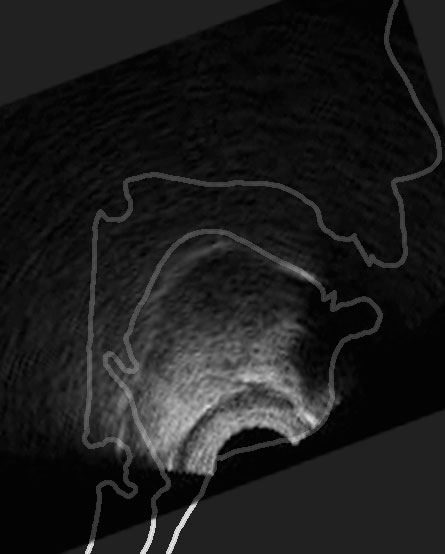
\includegraphics[width=.49\textwidth]{figures/DA_and_P1_overlay.jpg}
  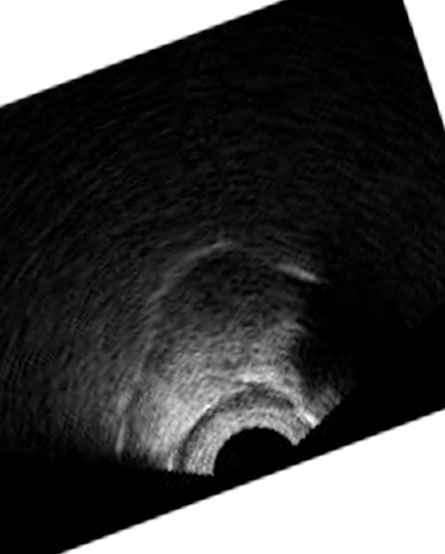
\includegraphics[width=.49\textwidth]{figures/DA_and_P1_overlay_3.jpg}
}

\frame{
  \centering
  {
    \vfill
    \bf \Large 
    \usebeamercolor[fg]{title}
    Projekti- ja tutkimuskohde-esimerkkejä
    \vfill
  }
}

% \item Tommi Nieminen \& Pertti Palo: Suomen \v{s}vaan artikulaatio.
% \begin{itemize}
% \item Aineistossa suomen lauseita epenteettisellä vokaalilla ja
%   ilman.
% \item Pieni pilottiaineisto: Yksi epäluotettava puhuja.
% \item Hyvä aika- ja paikkaresoluutio, kuvat selkeitä.
% \end{itemize}

\frame{\frametitle{Esimerkkiprojekti 1: Kliininen tutkimus}
  
\begin{itemize}
  \item Joanne Cleland \& al. - University of Strathclyde
  \begin{itemize}
    \item Kliinistä dataa kitahalkiopotilaiden post-operatiivisista
    kuntoutuskäynneistä.
    \item Tuloksia julkaistu eri muodoissa, mutta raakadata on suljettua.
    \item Hyvä aika- ja paikkaresoluutio, kuvien laatu vaihtelee paljon riippuen
    potilaan iästä ja muista tekijöistä.
    \item Lisähaasteena laitevian takia puuttuva synkroni ultraäänidatan ja
    audion välillä.
    \item Analyysi oli kuitenkin mahdollista valitsemalla videon perusteella
    maksimaaliset konsonanttiartikulaatiot analysoitavaksi.
    \item Lisäksi audion kohdistus ilmeisesti onnistui myös neuroverkkojen
    avulla myöhemmin.
    \end{itemize}
\end{itemize}
}

\frame{\frametitle{Esimerkkiprojekti 2: Koartikulaatiotutkimusta}

\begin{itemize}
\item Sonja Dahlgren, Pertti Palo \& Minnaleena Toivola: Kielten
koartikulaatiotyyppien kartoitusta.
  \begin{itemize}
  \item Aineistossa kielestä riippuen sanoja ja epäsanoja.
  \item Sekä muiden dataa että uutta .
  \item Hyvä aika- ja paikkaresoluutio, kuvat kohtuullisen selkeitä.
  \end{itemize}
\item Projektin tarkoitus on louda luokittelujärjestelmä eri kielten
koartikulaatiotavoille eli kuvata kuinka vokaalit ja konsonantit yhteistuotetaan
osana puhevirtaa.
\item Tähän aiheeseen erinomainen menetelmä on katsoa kielen pinnan asentoa
erottamalla se ultraäänikuvista splineillä. 
\end{itemize}
}

\frame{\frametitle{Splinit I}
  \hspace*{-.5cm}
  \centering
  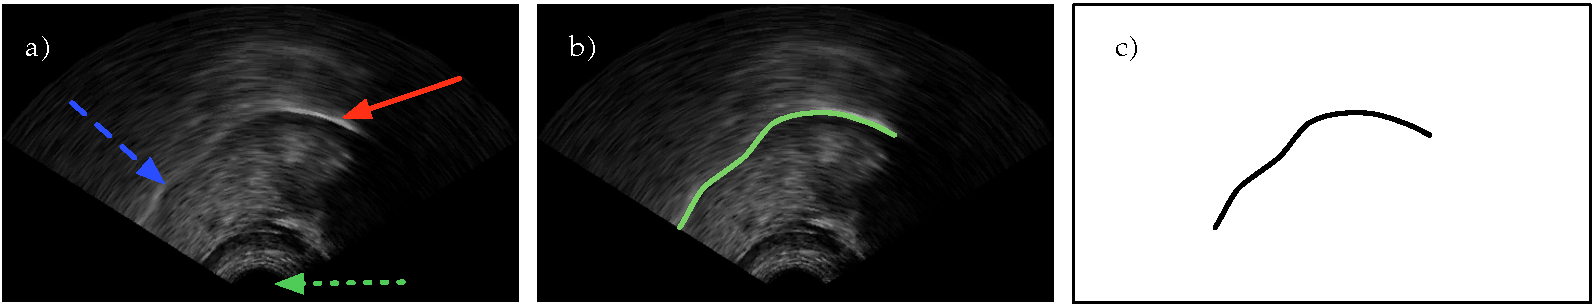
\includegraphics[width=1.05\textwidth]{P2_lemon_1st_frame_spline.pdf}
  \hspace*{.5cm}
  \begin{itemize}
  \item Splinin sovitus ultraäänikuvaan tarkoittaa, että piirrämme kielen pinnan
    mukaisen käyrän ultraäänikuvaan - tai oikeastaan asetamme splinin
    ohjauspisteet niin että splini asettuu kielen pinnan kohdalle.
  \item Sovitus voidaan tehdä joko manuaalisesti tai automaattisesti.
  \item Nykyisin automaattinen menetelmä on taitavan ihmisen tasolla useimmissa
  aineistoissa.
  \item Automaattista tulosta voidaan myös korjata manuaalisesti.
  \end{itemize}
}

\frame{\frametitle{Splinit II}

\begin{itemize}
  \item Tulokset riippuvat paljon datan laadusta:
  \begin{itemize}
    \item Parempi paikkaresoluutio auttaa, mutta ei takaa, sovittamisen
    onnistumista.
    \item Selkeisiin kuviin on helpompi sovittaa splini.
  \end{itemize}
  \item Splinit itsessään voivat olla analyysin tulos ja niitä voidaan
  verrata toisiinsa silmämääräisesti.
  
\end{itemize}
}

\frame{\frametitle{Esimerkkiprojekti 2: Koartikulaatiotutkimusta}

\begin{center}
  \hspace*{-.85cm}
  \includegraphics[width=1.15\textwidth]{figures/greek_vs_finnish_vs_italian_vs_gam.drawio.png}
\end{center}

\begin{itemize}
\item Tässä on hyvä esimerkki siitä miten pääefekti voi olla näkyvissä suoraan
pienessäkin datassa.
\end{itemize}
}


\frame{\frametitle{Esimerkkiprojekti 3: Arabian konsonantteja}

  \begin{itemize}
    \item Jalal Al-Tamimi \& Pertti Palo (forthcoming): ``Tongue
    contours in guttural consonants in Levantine Arabic: A Generalised
    Additive Modelling Approach''
    \begin{itemize}
    \item Aineistossa levantin arabinkielisiä sanoja.
    \item Laaja julkaisuihin tähtäävä aineisto: Puhujia kaikkiaan 10.
    \item Hyvä aikaresoluutio, paikkaresoluutio heikompi. Kuvat
      vähemmän selkeitä.
    \end{itemize}
  \end{itemize}
  }
  
\frame{\frametitle{Esimerkkiprojekti 3}
  
    \begin{itemize}
      \item Alla analyysituloksia jotka esiteltiin ISSP 2020-konferenssisa. 
      \item Kuvissa y-akseli on aika (alhaalta ylös), x-akseli on paikka
      vasen-oikea = takana-edessä, ja vaalea väri tarkoittaa korkeampaa kielen
      asentoa, punaisempi/tummempi matalempaa.    
    \end{itemize}
    \begin{center}
      \includegraphics[width=.9\textwidth]{figures/jalal_2D_diff.png}
    \end{center}
}

\frame{
  \centering
  {
    \vfill
    \bf \Large 
    \usebeamercolor[fg]{title}
    Lyhyt tauko (5 min)
    \vfill
  }
}

\frame{\frametitle{Esimerkkiprojekti 4: Kurkunpään liikkeitä}
  
  \begin{itemize}
    \item Scott R. Moisik, Hua Lin and John H. Esling (2014). A
    study of laryngeal gestures in Mandarin citation tones using simultaneous
    laryngoscopy and laryngeal ultrasound (SLLUS) . Journal of the International
    Phonetic Association, 44, pp 21-58 doi:10.1017/S0025100313000327
    \item Vent = valeäänihuuli, VF = äänihuuli, AE = aryepiglottaalinen poimu, P = anturi.
  \end{itemize}

  \hspace*{-.5cm}
  \begin{center}
    \includegraphics[width=1\textwidth]{figures/larynx_probe_placement.png}
  \end{center}
}

\frame{\frametitle{Kurkunpään ultraääni - anturivaihtoehtoja}
  \begin{center}
    \includegraphics[width=0.5\textwidth]{figures/fan_vs_linear.png}
  \end{center}

  \begin{itemize}
    \item Samat rakenteet, erilainen anturi -> erilainen kuva.
  \end{itemize}
  {\scriptsize Kuvat: Moisik, S. R., Esling, J. H., Bird, S., \& Lin, H. (2011). Evaluating
  laryngeal ultrasound to study larynx state and height. In W. S. Lee \& E. Zee
  (Eds.), Proceedings of the 17th International Congress of Phonetic Sciences
  (pp. 136 -- 139).}
}

\frame{\frametitle{Esimerkkiprojekti 4: Kurkunpään liikkeitä}
  
  \begin{center}
    \includegraphics[width=0.9\textwidth]{figures/optic_flow.png}
  \end{center}

  \begin{itemize}
    \item Moisik, S. R., Esling, J. H., Bird, S., \& Lin, H. (2011). Evaluating
    laryngeal ultrasound to study larynx state and height. In W. S. Lee \& E.
    Zee (Eds.), Proceedings of the 17th International Congress of Phonetic
    Sciences (pp. 136 -- 139).
  \end{itemize}

  }


\frame{\frametitle{Esimerkkiprojekti 5: Äänettömän artikulaation kartoitusta}

  \begin{itemize}
  \item Pertti Palo: Puhunnosten alkujen ajoitusta - väitöskirjadataa.
    \begin{itemize}
    \item Aineistossa skottienglannin leksikaalisia /CVC/-sanoja.
    \item Väitöskirjan päädata.
    \item Erinomainen aika- ja paikkaresoluutio, kuvat selkeitä.
    \end{itemize}
  \end{itemize}
  }  

\frame{\frametitle{Pikselietäisyys: Raakadata}
  \hspace*{-.5cm}
  \centering
  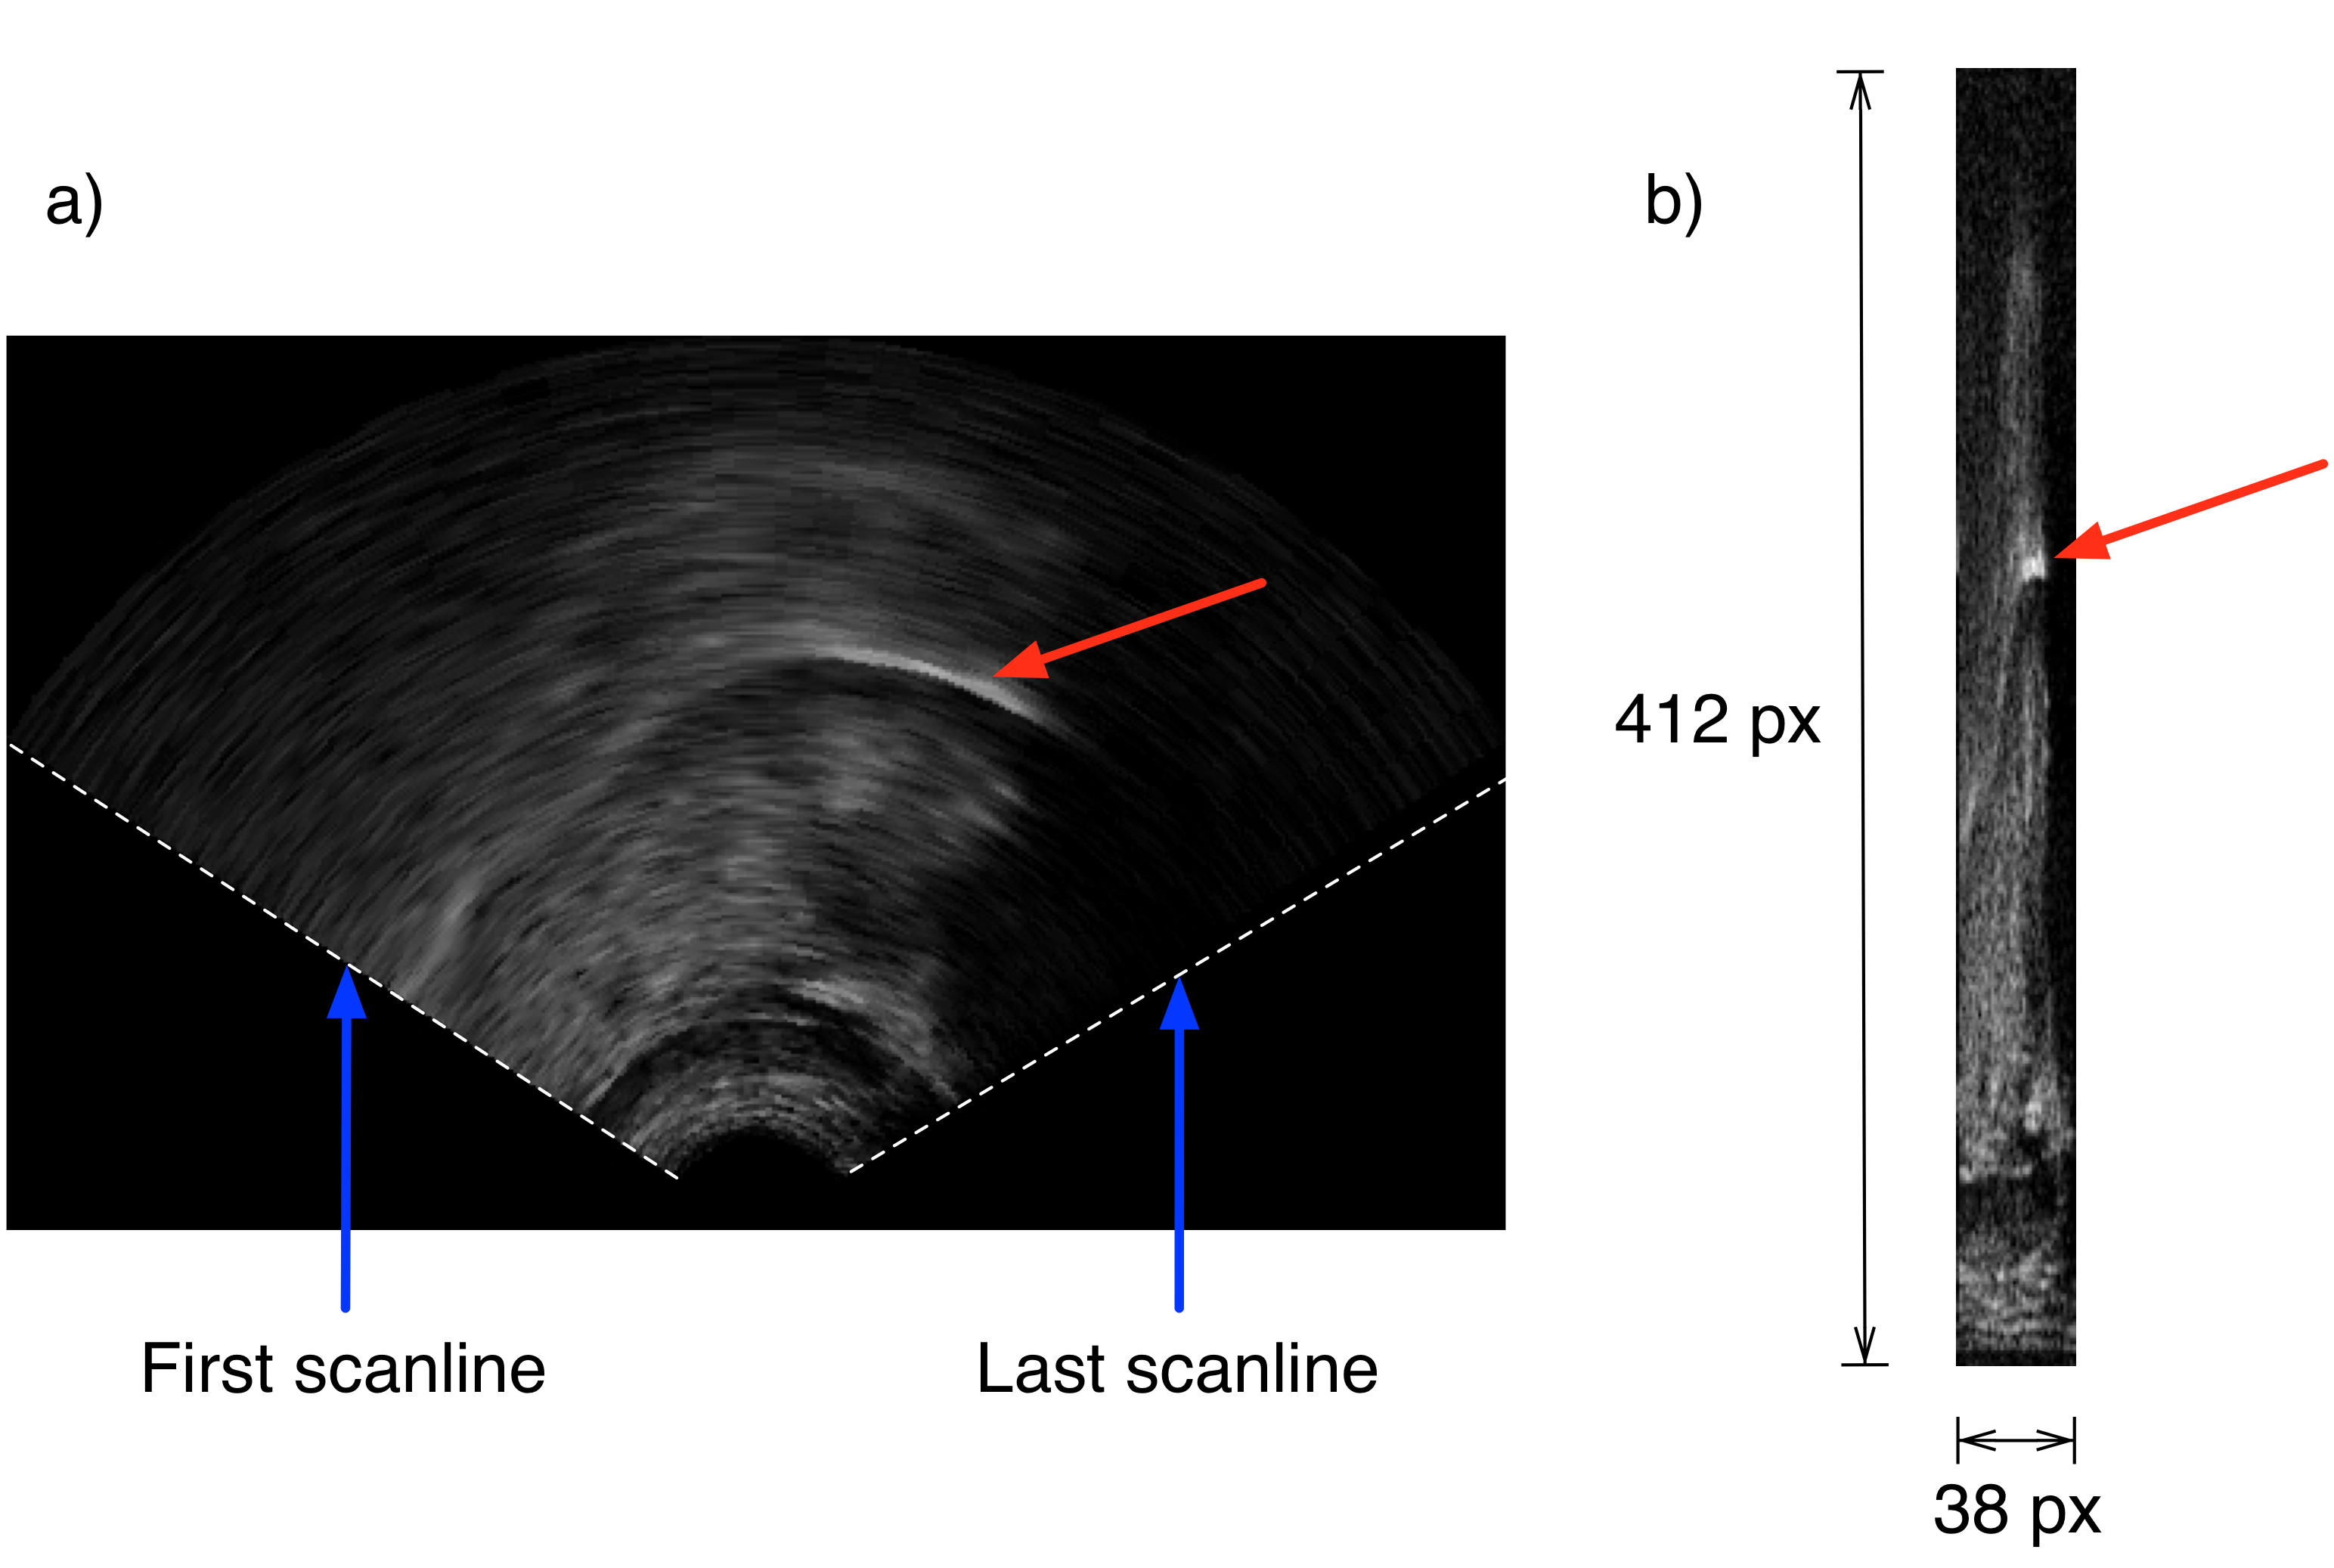
\includegraphics[width=1.05\textwidth]{P2_lemon_1st_frame_fan_v2.jpg}
}

\frame{\frametitle{Pikselietäisyys: Miten laskenta tapahtuu?}
  \hspace*{-.5cm}
  \centering
  \includegraphics[width=1.05\textwidth]{figures/pixel_difference_demo.pdf}
}

\frame{\frametitle{Pikselietäisyys: Missä liike alkaa?}
  \hspace*{-.5cm}
  \centering
  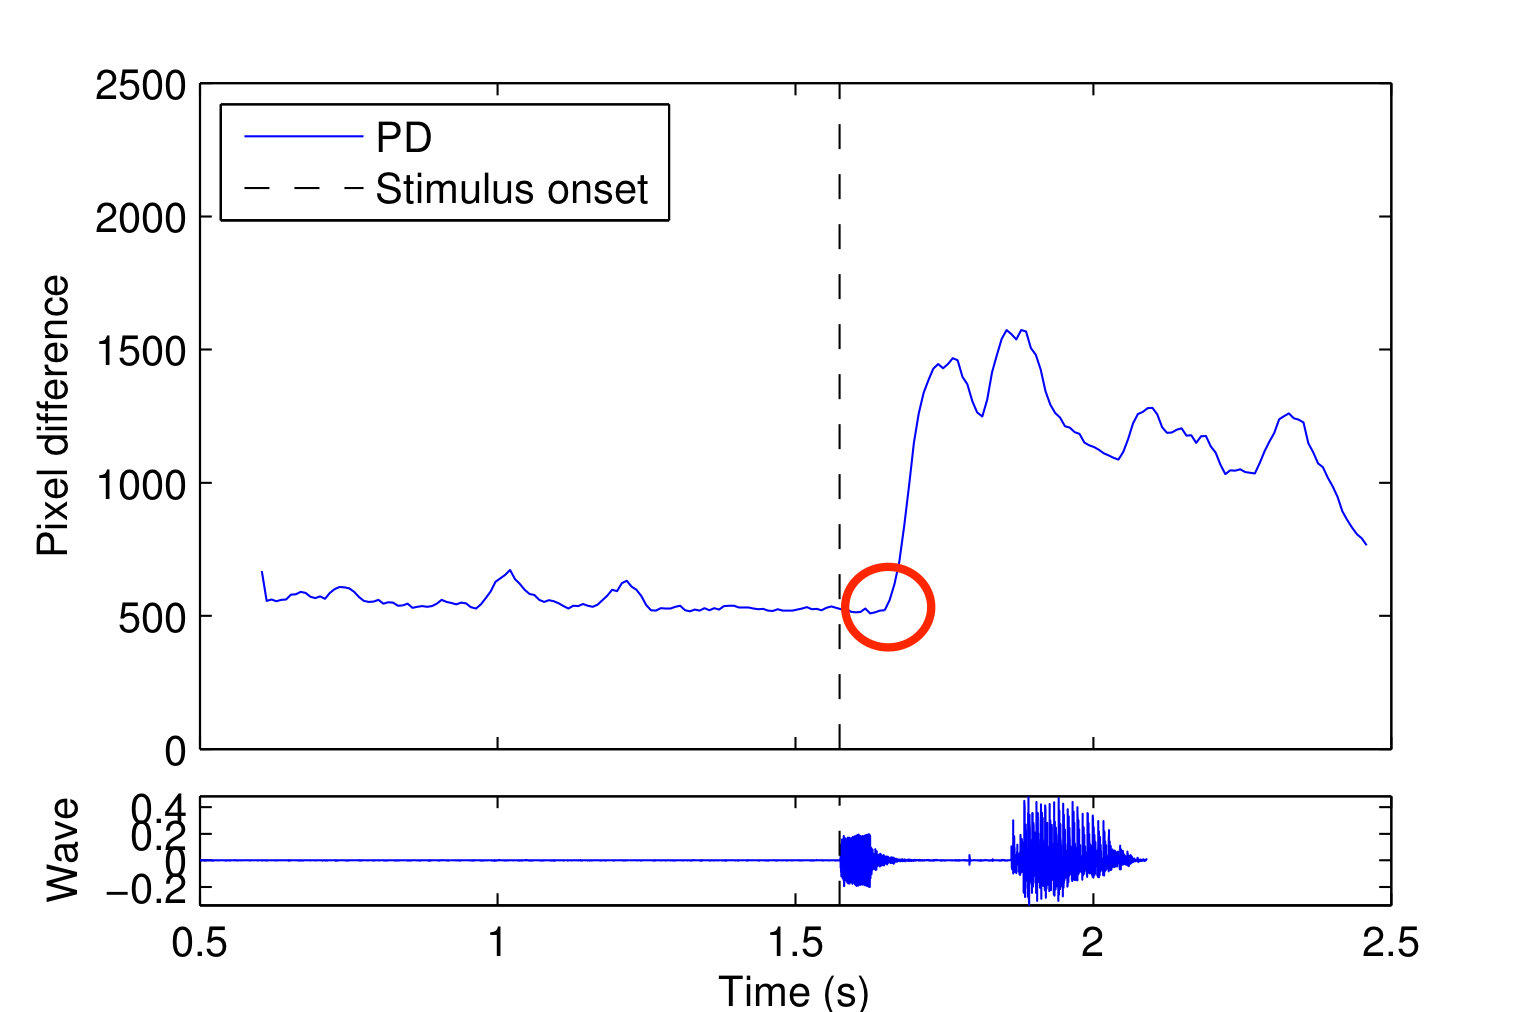
\includegraphics[width=\textwidth]{PD_annotated.jpg}
}



\frame{
  \centering
  {
    \vfill
    \bf \Large 
    \usebeamercolor[fg]{title}
    Analyysimenetelmiä
    \vfill
  }
}

\frame{\frametitle{Audio}
  \begin{itemize}
  \item Tärkeä osa dataa on ultraäänen kanssa yhdessä synkronoidusti
    tallennettu ääni.
  \item Ääntä voi analysoida AAA:lla, mutta se on helpompaa
    Praatilla.
  \item Akustisen segmentoinnin tuloksista on huomattavaa hyötyä
    aineiston rajaamisessa. Niiden avulla artikulatorinen analyysi
    voidaan kohdistaa vain siihen osaan tallenteita, mistä ollaan 
    kiinnostuneita.
  \end{itemize}
}

\frame{\frametitle{Artikulatorinen data}
  \begin{itemize}
  \item Keskitymme tällä kertaa kieliultraäänen analyysiin.
  \item On kuitenkin hyvä huomata, että myös muita datatyyppejä tai
    -modaliteetteja voidaan yleensä tallentaa samalla laitteistolla --
    pienillä tai suurilla muutoksilla:
    \begin{itemize}
    \item Kurkunpään ultraääni käyttää yleensä erityyppistä anturia,
      joka pitää ostaa erikseen. Datan analyysi on tyypillisesti hyvin
      erilaista kuin kieliultraäänen analyysi, koska rakenteet ovat
      paljon monimutkaisempia.
    \item Huulivideoita voidaan tallentaa helposti. HY:n laitteistolla
      niitä saadaan joko kasvojen sivulta tai edestä. Huulivideoiden
      analyysiin on myös olemassa työkaluja.
    \item Suurempaa työtä vaatii yhtäaikainen datan tallennus
      esim. ultraäänellä ja elektromagneettisella artikulografialla
      tai muilla menetelmillä.
    \end{itemize}
  \end{itemize}
}

\frame{\frametitle{Pelkät videot tai kuvat}
  \begin{itemize}
  \item Ultraäänivideoita voidaan annotoida siinä missä mitä hyvänsä
    videoita.
  \item Työ ei ole ihan kevyttä, joten aiheen ja materiaalin
    rajauksessa kannattaa olla huolellinen.
  \item Annotoinnin voi tehdä AAA:lla tai vaikkapa
    .avi-tiedostoiksi tallenettuja videoita voi käsitellä videoiden
    annotointiin tarkoitetuilla ohjelmilla.
  \item Yksittäisistä kuvista voi myös tehdä suoria mittauksia.
  \end{itemize}
}

% \frame{\frametitle{Splinit III: Lähempi esimerkki}

% \hspace*{-.5cm}
%   \centering
%   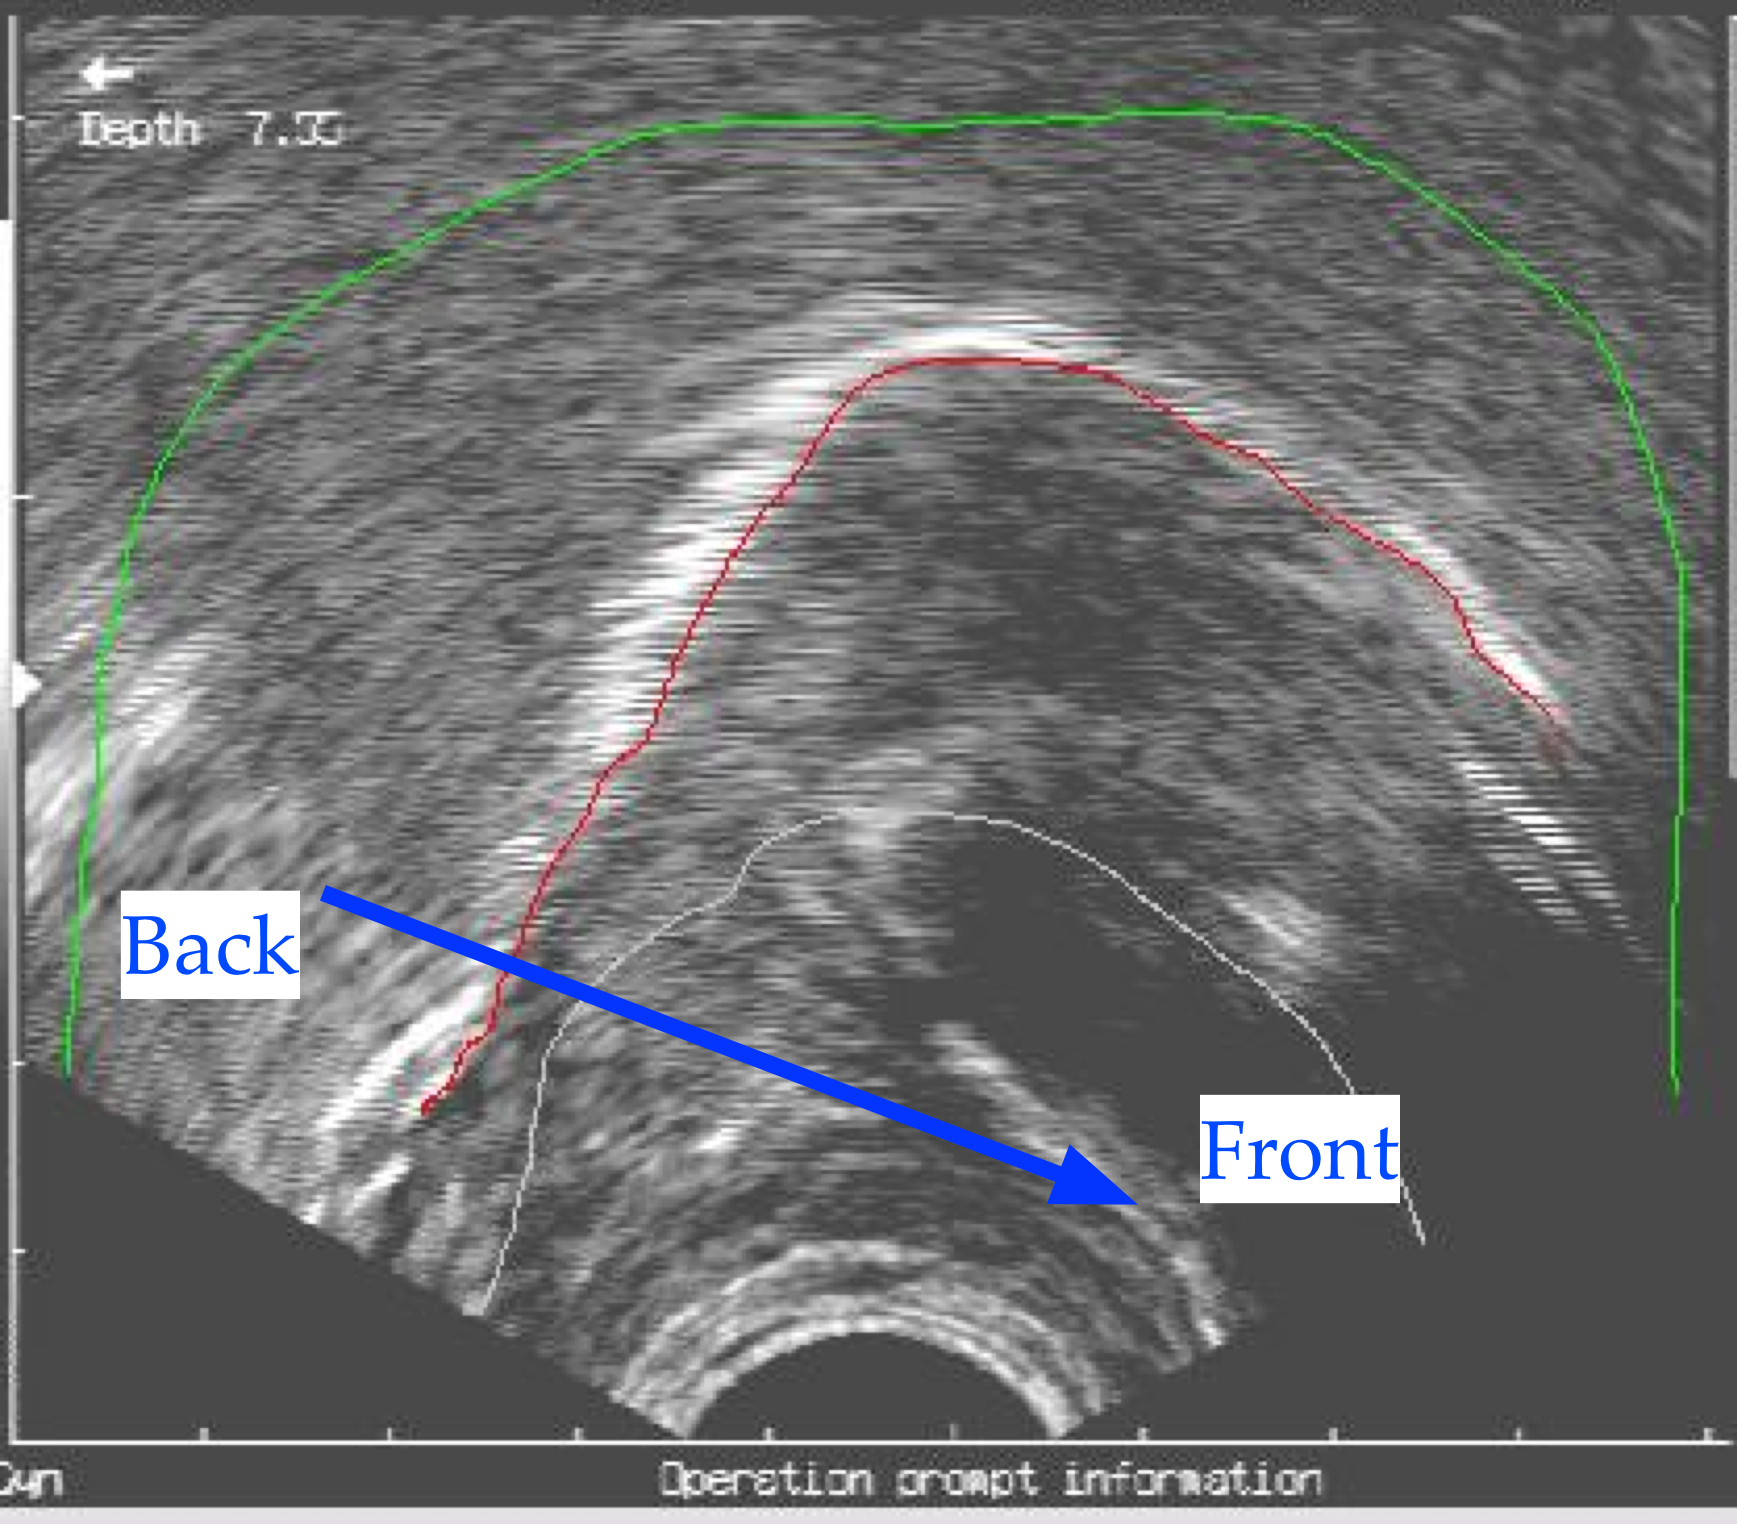
\includegraphics[width=.7\textwidth]{uti_traced}
% }

% \frame{\frametitle{Splinit IV: Analyysimenetelmiä}
%   \hspace*{-.45cm}
%   \centering
%   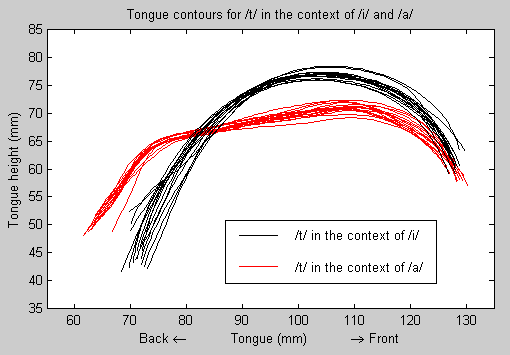
\includegraphics[width=.8\textwidth]{uti_contours}
%   \vfill
%   Perinteinen menetelmä: Valitaan audiosegmentaation perusteella
%   ajasta kaksi tai useampia mielenkiintoisia pisteitä ja verrataan
%   splinien muotoa niissä.
% }
  
\frame{\frametitle{Splinien analyysimenetelmiä}

  \hspace*{-.45cm}
  \centering
  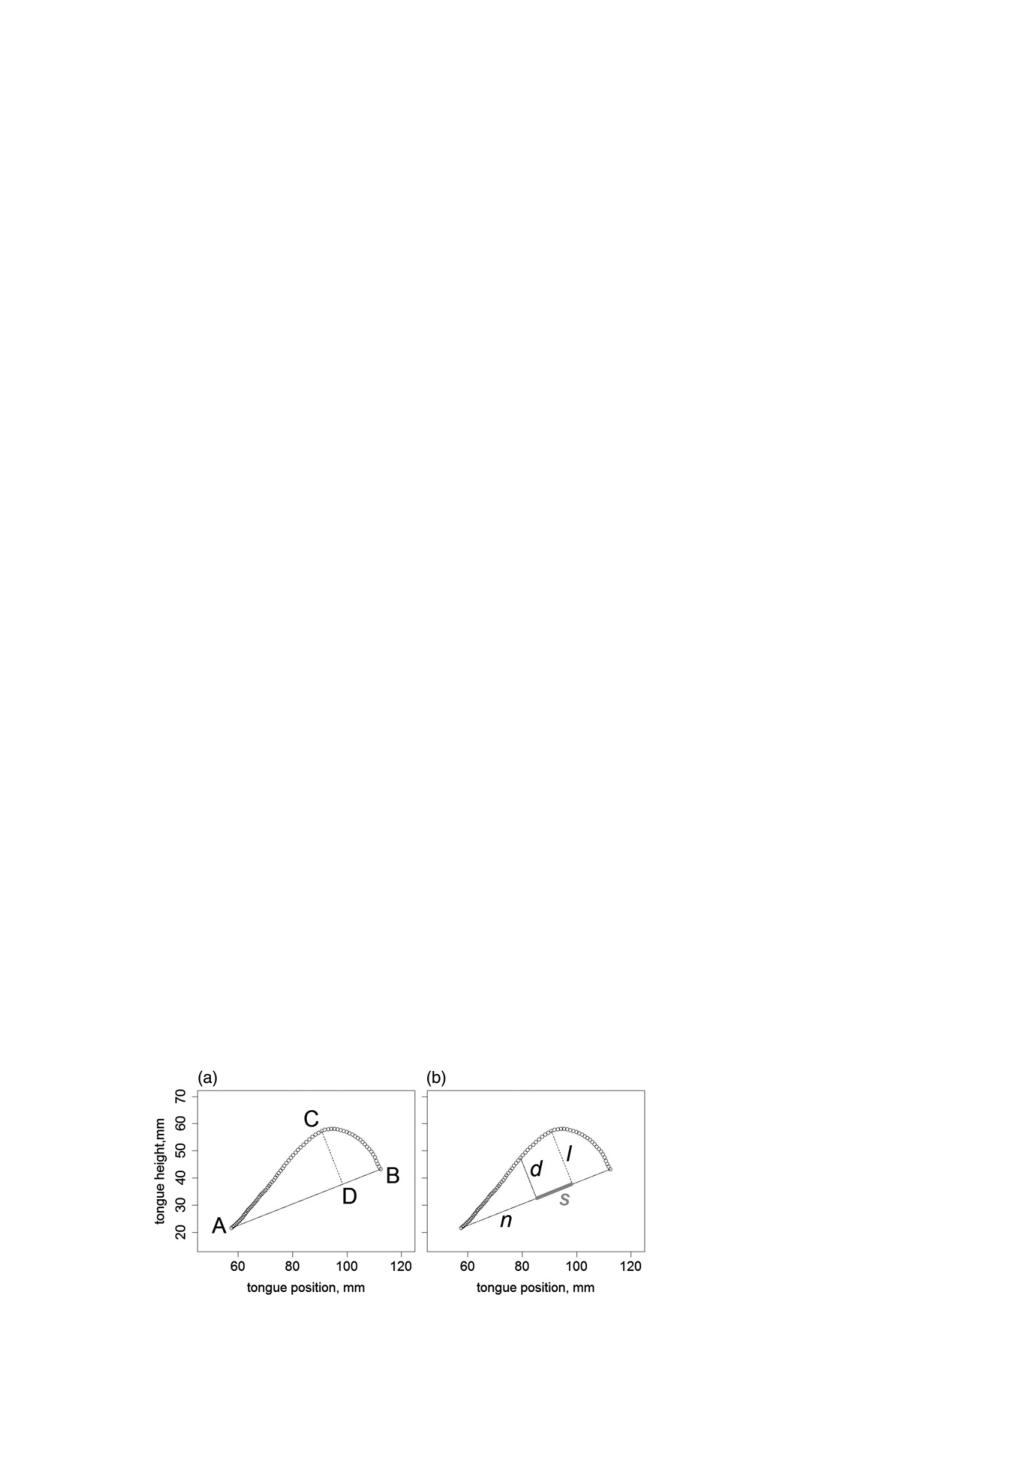
\includegraphics[width=.8\textwidth]{zharkova_metrics.pdf}

  \begin{itemize}
  \item Splinien muotoa voidaan analysoida myös ajan funktiona
    funktionaalisella data analyysilla ilman tarvetta rajoittua
    yksittäisiin ajanhetkiin analyysissä.
  \item Splineistä voidaan myös laskea erilaisia metriikoita ja
    verrata niitä sitä kautta toisiinsa. Esimerkiksi
    \cite{Zharkova:QLC:2015}.
  \item Menetelmiä on paljon ja erilaisiin kysymyksiin sopivat eri
    menetelmät.
  \end{itemize}
}

\frame{\frametitle{Laskennalliset metriikat}
  \begin{itemize}
  \item Voimme myös analysoida videoiden informaatiosisältöä
    erottamatta niistä kielenpintaa tai muita anatomisia
    rakenteita. Esimerkiksi:
    \begin{itemize}
    \item Pikselietäisyys (engl. Pixel Difference / PD, seuraavat
      kalvot) seuraa kokonaismuutosta ultraäänen raakadatan
      perusteella. Sopii erityisen hyvin liikkeen alun paikantamiseen.
    \item Optinen virta (engl. Optic flow) seuraa kuvan osien liikettä
      tilastollisin menetelmin ja arvioi mihin päin kuvan eri osat
      liikkuvat. Tämä on tärkeä menetelmä kurkunpään ultraäänen
      analyysissa.
    \item Kuvasarjojen suora tilastollinen analyysi
      \cite{Saito:USF:2020}.
    \end{itemize}
  \item Näitä ja muita menetelmiä voidaan käyttää myös splinien
    rinnalla tuomassa lisätietoa.
  \end{itemize}
}

\frame{
  \centering
  {
    \vfill
    \bf \Large 
    \usebeamercolor[fg]{title}
    Kyselkää
    \vfill
  }
}


\frame{\frametitle{Kirjallisuutta ja kiitokset}
  \nocite{AlTamimi:TCG:2022,Dahlgren:SLS:2022,Palo:MPS:2019}
  
  \begin{itemize}
  \item Steve Cowen: AAA:n käyttöapu ja kuva minusta.
  \item Felix Schaeffler: lepakkokuva.
  \item Alan Wrench: AAA:n käyttöapu ja laitteistokuvat.
  \end{itemize}
  
  \vspace*{.5cm}

  {\tiny
    \bibliographystyle{apalike}
    \bibliography{bib/master,bib/jpalo}
  }
}


% \frame{\frametitle{Analyysiesimerkki koartikulaatiodatasta}

%   \begin{itemize}
%   \item Segmentoidaan audio.
%   \item Valitaan mielenkiintoiset kohdat.
%   \item Splinitetään mielenkiintoiset kohdat.
%   \item Korjataan splinit käsin.
%   \item Lopuksi tehtäisiin AAA:ssa/R:ssä/Pythonilla splinianalyysia,
%     mutta ei mennä niin pitkälle tänään.
%   \end{itemize}
% }


\end{document}

